%% fcup-thesis.tex -- document template for PhD theses at FCUP
%%
%% Copyright (c) 2015 João Faria <joao.faria@astro.up.pt>
%%
%% This work may be distributed and/or modified under the conditions of
%% the LaTeX Project Public License, either version 1.3c of this license
%% or (at your option) any later version.
%% The latest version of this license is in
%%     http://www.latex-project.org/lppl.txt
%% and version 1.3c or later is part of all distributions of LaTeX
%% version 2005/12/01 or later.
%%
%% This work has the LPPL maintenance status "maintained".
%%
%% The Current Maintainer of this work is
%% João Faria <joao.faria@astro.up.pt>.
%%
%% This work consists of the files listed in the accompanying README.

%% SUMMARY OF FEATURES:
%%
%% All environments, commands, and options provided by the `ut-thesis'
%% class will be described below, at the point where they should appear
%% in the document.  See the file `ut-thesis.cls' for more details.
%%
%% To explicitly set the pagestyle of any blank page inserted with
%% \cleardoublepage, use one of \clearemptydoublepage,
%% \clearplaindoublepage, \clearthesisdoublepage, or
%% \clearstandarddoublepage (to use the style currently in effect).
%%
%% For single-spaced quotes or quotations, use the `longquote' and
%% `longquotation' environments.


%%%%%%%%%%%%         PREAMBLE         %%%%%%%%%%%%

%%  - Default settings format a final copy (single-sided, normal
%%    margins, one-and-a-half-spaced with single-spaced notes).
%%  - For a rough copy (double-sided, normal margins, double-spaced,
%%    with the word "DRAFT" printed at each corner of every page), use
%%    the `draft' option.
%%  - The default global line spacing can be changed with one of the
%%    options `singlespaced', `onehalfspaced', or `doublespaced'.
%%  - Footnotes and marginal notes are all single-spaced by default, but
%%    can be made to have the same spacing as the rest of the document
%%    by using the option `standardspacednotes'.
%%  - The size of the margins can be changed with one of the options:
%%     . `narrowmargins' (1 1/4" left, 3/4" others),
%%     . `normalmargins' (1 1/4" left, 1" others),
%%     . `widemargins' (1 1/4" all),
%%     . `extrawidemargins' (1 1/2" all).
%%  - The pagestyle of "cleared" pages (empty pages inserted in
%%    two-sided documents to put the next page on the right-hand side)
%%    can be set with one of the options `cleardoublepagestyleempty',
%%    `cleardoublepagestyleplain', or `cleardoublepagestylestandard'.
%%  - Any other standard option for the `report' document arclass can be
%%    used to override the default or draft settings (such as `10pt',
%%    `11pt', `12pt'), and standard LaTeX packages can be used to
%%    further customize the layout and/or formatting of the document.

%% *** Add any desired options. ***
%PDF
%\documentclass[a4paper,narrowmargins,11pt,oneside,draft,onehalfspaced,singlespacednotes]{fcup-thesis}
%\documentclass[a4paper,narrowmargins,11pt,oneside,onehalfspaced,singlespacednotes]{fcup-thesis}
%Print
%\documentclass[draft,a4paper,narrowmargins,11pt,twoside,openright,onehalfspaced,singlespacednotes]{fcup-thesis}
\documentclass[a4paper,narrowmargins,11pt,twoside,openright,onehalfspaced,singlespacednotes]{fcup-thesis}

%% *** Add \usepackage declarations here. ***
%% The standard packages `geometry' and `setspace' are already loaded by
%% `ut-thesis' -- see their documentation for details of the features
%% they provide.  In particular, you may use the \geometry command here
%% to adjust the margins if none of the ut-thesis options are suitable
%% (see the `geometry' package for details).  You may also use the
%% \setstretch command to set the line spacing to a value other than
%% single, one-and-a-half, or double spaced (see the `setspace' package
%% for details).


%%%%%%%%%%%%%%%%%%%%%%%%%%%
% Overfull statements fix %
%%%%%%%%%%%%%%%%%%%%%%%%%%%
\pretolerance=150
\setlength{\emergencystretch}{3em}

%%%%%%%%%%%%%%%%%%%%%%%%%%
% Standard british babel %
%%%%%%%%%%%%%%%%%%%%%%%%%%
\usepackage[english]{babel}

% Enable array for text formatting 
\usepackage{array}

% Standard Mathematics library 
\usepackage{amsmath}  

% Standard symbols for asmath library
\usepackage{amssymb}

%%%%%%%%%%%%%%%%%%%%%%%%%%%%%%%%%%%%%%%%%%%
% Override the basic math font with arial %
%%%%%%%%%%%%%%%%%%%%%%%%%%%%%%%%%%%%%%%%%%%
% Math font specification package
\usepackage{mathspec}

% Proporitional lining for digits latin and greek letters
\setmathsfont(Digits)[Numbers={Lining,Proportional}]{Arial}
\setmathsfont(Latin)[Numbers={Lining,Proportional}]{Arial}
\setmathsfont(Greek)[Numbers={Lining,Proportional}]{Arial}

% Main direction symbols for integrals derivations etc
\usepackage{mdsymbol}

% asmath symbols and additional library
\usepackage{amsthm}      

% Enable usage of Eulerscript for special math symbols
\usepackage[mathscr]{euscript}

%%%%%%%%%%%%%%
% Algorithms %
%%%%%%%%%%%%%%
% Enable algorithms - nice format use chapter numbering
\usepackage[ruled,algochapter]{algorithm2e}

% custom keywords for alggorithms
\usepackage{algorithmic}

%%%%%%%%
% Misc %
%%%%%%%%
% Enable bold symbols in math mode (unused ?)
\usepackage{bm}

% Enhanced support for graphics (ugly hack on big schemes)
\usepackage{graphicx}       

% Replace strings in encapsulated PostScript figures (Arial to my PS files ...)
\usepackage{psfrag}         

% Sophisticated verbatim text (nice notes and foootnotes)
\usepackage{fancyvrb}    

%Im­proves the in­ter­face for defin­ing float­ing ob­jects such as fig­ures and ta­bles. In­tro­duces the boxed float, the ruled float and the plain­top float. You can de­fine your own floats and im­prove the be­haviour of the old ones.  The pack­age also pro­vides the H float mod­i­fier op­tion of the ob­so­lete here pack­age. You can se­lect this as au­to­matic de­fault with \float­place­ment{fig­ure}{H}. (Nice floats and fixed figures/algorithms/equations).
\usepackage{float}

%Mod­i­fies the tab­u­larx en­vi­ron­ment to com­bine the fea­tures of the tab­u­larx pack­age (auto-sized columns in a fixed width ta­ble) with those of the longtable pack­age (multi-page ta­bles). 
\usepackage{ltablex}

%Library bibtex wrapper, square brackets, sort by first author surname, use coma seprarator, use number labeling
\usepackage[square,sort,comma,numbers]{natbib}        

%A sym­bol font (dis­tributed as METAFONT source) that con­tains many of the sym­bols of the Zapf ding­bats set, to­gether with an NFSS in­ter­face for us­ing the font.
\usepackage{bbding}

%The dcol­umn pack­age makes use of the ar­ray pack­age to de­fine a "D" col­umn for­mat for use in tab­u­lar en­vi­ron­ments. (Multicollumn enviroment , layered tables)
\usepackage{dcolumn}        

%The pack­age en­hances the qual­ity of ta­bles in LATEX, pro­vid­ing ex­tra com­mands as well as be­hind-the-scenes op­ti­mi­sa­tion. Guide­lines are given as to what con­sti­tutes a good ta­ble in this con­text. From ver­sion 1.61, the pack­age of­fers longtable com­pat­i­bil­ity. (Yet another table hacks)
\usepackage{booktabs} 

%The pack­age has a lot of flex­i­bil­ity, in­clud­ing an op­tion for spec­i­fy­ing an en­try at the “nat­u­ral” width of its text. (Multirow cells in table headres)
\usepackage{multirow}

%Pro­vides enu­mer­ate and item­ize en­vi­ron­ments that can be used within para­graphs to for­mat the items ei­ther as run­ning text or as sep­a­rate para­graphs with a pre­ced­ing num­ber or sym­bol. (Nice paragraph/itemize/enumerate) package
\usepackage{paralist}     

%Draft only enviromental enabler (Deprecated - for table debug mainly)
\usepackage{ifdraft}  

% indentfirst – Indent first paragraph after section header by default disabled 
%\usepackage{indentfirst}    

% Add bibliography/index/contents to Table of Contents (\bibliography{*} command)
\usepackage[nottoc,notlof,notlot]{tocbibind}

% Pretty and clickable urls in 
\usepackage{url}

% multiline collumn tables (Nomenclature)
\usepackage{tabularx}

%%%%%%%%%%%%%%%%%%%%%%%%%%%%%%%%%%%
% Table figure caption subcaption %
%%%%%%%%%%%%%%%%%%%%%%%%%%%%%%%%%%%
% use font size for captions like 8pt -> normalisize 11pt, scriptsize->8pt
\usepackage[font={scriptsize}]{caption}

% use font size for captions like 8pt -> normalisize 11pt, scriptsize->8pt
\usepackage[font={scriptsize}]{subcaption}

% Other packages caption setup, just for ensurance
\captionsetup{font=scriptsize}

% Hypper references - clickable labels 
\usepackage[unicode]{hyperref}

% Specific color package - color by name hex, cmyk etc.
\usepackage{xcolor}

%%%%%%%%%%%%%%%%%%%%%%%%%%%%%%%%%%
% Document setup for referencing %
%%%%%%%%%%%%%%%%%%%%%%%%%%%%%%%%%%
\hypersetup{pdftitle=Obstacle Avoidance Framework based on Reach Sets, 
            pdfauthor=Alojz Gomola,
            colorlinks=false,
            urlcolor=blue,
            pdfstartview=FitH,
            pdfpagemode=UseOutlines,
            pdfnewwindow,
            breaklinks
          }
%%%%%%%%%%%%%%%%%%%%%%          
%% Arrays in tables %%
%%%%%%%%%%%%%%%%%%%%%%       
% Array package import
\usepackage{array}

% Left alignement
\newcolumntype{L}[1]{>{\raggedright\let\newline\\\arraybackslash\hspace{0pt}}m{#1}}

% Center alignement
\newcolumntype{C}[1]{>{\centering\let\newline\\\arraybackslash\hspace{0pt}}m{#1}}

% Right alignement
\newcolumntype{R}[1]{>{\raggedleft\let\newline\\\arraybackslash\hspace{0pt}}m{#1}}         

% Multiline column with text filling
\newcolumntype{B}{X}

% Multiline column with X percentage of text width
\newcolumntype{S}[1]{>{\hsize=#1\textwidth}X}

% twoline cell definition macro
\newcommand{\twolinecellr}[2][r]{%
  \begin{tabular}[#1]{@{}r@{}}#2\end{tabular}}

% Section state macro - deprecated used during writting of thesis
\newcommand{\secState}[1]{
	\ifdraft{(#1) }{}
}

%%%%%%%%%%%%%%%%%%%%
% Figure directory %
%%%%%%%%%%%%%%%%%%%%
\newcommand{\FIGDIR}{./Pics}    %%% directory containing figures

%%%%%%%%%%%%%%%%%%%%%%%%%%%%%%%%%%%%%%%%%%%%%%%%
% Theorems/defs and other structured referables%
%%%%%%%%%%%%%%%%%%%%%%%%%%%%%%%%%%%%%%%%%%%%%%%%
% Plain style of theorems - inline in text
\theoremstyle{plain}

% Theorem keyword definition
\newtheorem{theorem}{Theorem}

% Lemma for theorem keyword definition
\newtheorem{lemma}[theorem]{Lemma}

% Proposition for theorem keyword definition 
\newtheorem{proposition}[theorem]{Proposition}

% If different theorem type for proof/problem/definition is required
\theoremstyle{plain}

% Definition keyword
\newtheorem{definition}{Definition}

% Problem keyword
\newtheorem{problem}{Problem}

% Example keyword
\newtheorem{example}{Example}

% Assumnption keyword
\newtheorem{assumption}{Assumption}

% Remark style without numbering
\theoremstyle{remark}

% Corollary keyword definition
\newtheorem*{corollary}{Corollary}
% Note keyword definition
\newtheorem*{note}{Note}

%Proof of the theorem, without numbering (discontinued)
\newenvironment{dokaz}{
  \par\medskip\noindent
  \textit{Proof}.
}{
\newline
\rightline{\SquareCastShadowBottomRight}
}

%Contraint of the theorem/proof numbering (discontinued)
\newenvironment{constraints}[1]{
  \par\medskip\noindent
  \textit{Constraints #1} \\
}{
\newline
\rightline{\SquareCastShadowBottomRight}
}

%%%%%%%%%%%%%%%%%%%%%%%%%%%%%%%%%%%%%%
%% Additional bibliography settings %%
%%%%%%%%%%%%%%%%%%%%%%%%%%%%%%%%%%%%%%
%\bibliographystyle{plainnat}     %% Author (year) style
\bibliographystyle{unsrt}        %% [number] style
\setcitestyle{square}

%%%%%%%%%%%%%%%%%%%%%%%%%%%%%%%
% Section  4.7 Challenge list %
%%%%%%%%%%%%%%%%%%%%%%%%%%%%%%%
\newif\ifproblemchallenge   %# Build block for problem challenges
\problemchallengetrue       %# Show comments

%%%%%%%%%%%%%%%%%%%%%%%%%%
%% Custom Math commands %%
%%%%%%%%%%%%%%%%%%%%%%%%%%
% Real numbers set
\newcommand{\R}{\mathbb{R}}

% Natural numbers set
\newcommand{\N}{\mathbb{N}}

% Natural distribution
\DeclareMathOperator{\pr}{\textsf{P}}

% Euclid distribution
\DeclareMathOperator{\E}{\textsf{E}\,}

% Standard derivation
\DeclareMathOperator{\var}{\textrm{var}}

% Variation
\DeclareMathOperator{\sd}{\textrm{sd}}

% Top description
\newcommand{\T}[1]{#1^\top}        

% Reference 
\newcommand{\goto}{\rightarrow}

% Reference top
\newcommand{\gotop}{\stackrel{P}{\longrightarrow}}

% Average complexity of algorithm
\newcommand{\maon}[1]{o(n^{#1})}

% absolute value of compbound equation
\newcommand{\abs}[1]{\left|{#1}\right|}

% Inverted sqare of the value
\newcommand{\isqr}[1]{\frac{1}{\sqrt{#1}}}

% Norm of the compobound equation
\newcommand{\norm}[1]{\left\lVert#1\right\rVert}

% random distribution box
\newcommand{\pulrad}[1]{\raisebox{1.5ex}[0pt]{#1}}

% another ugly multicolum in equation
\newcommand{\mc}[1]{\multicolumn{1}{c}{#1}}

% To be done block in red collor only in draft mode
\newcommand{\TBD}[1]{\color{red}\emph{--TBD:}#1\color{black}}

%%%%%%%%%%%%%%%%%%%%%%%%%%%%%%%%%%%%%%%%%%%%%%%%%%%%%%%%%%%%%%%%%%%%%%
% Set arial as default font using MS word 2003 Arial font definition %
%%%%%%%%%%%%%%%%%%%%%%%%%%%%%%%%%%%%%%%%%%%%%%%%%%%%%%%%%%%%%%%%%%%%%%
\usepackage{fontspec}
\setmainfont[
	Path={fonts/},
	UprightFont=*-Regular,
	ItalicFont=*-Italic,
	BoldFont=*-Bold,
	BoldItalicFont=*-Bold-Italic
]{Arial}

%%%%%%%%%%%%%%%%%%%%%%%%
% Renew title section  %
%%%%%%%%%%%%%%%%%%%%%%%%
\usepackage{titlesec}

% Define special thick after header lines for chapter/section/subsection
\newcommand{\hchapterspoce}{\hspace{20pt}}
\newcommand{\hsectuibspoce}{\hspace{15pt}}
\newcommand{\hsubsectuibspoce}{\hspace{10pt}}

%Chapter hanger 20 pt
\titleformat{\chapter}[hang]{\Huge}{Chapter \thechapter.\hchapterspoce}{0pt}{\Huge}[{\titlerule[1pt]}]

%Section hanger 16 pt
\titleformat{\section}[hang]{\huge}{\thesection.\hsectuibspoce}{0pt}{\huge}[{\titlerule[0.7pt]}]

%Subsection hanger 14 pt
\titleformat{\subsection}[hang]{\Large}{\thesubsection.\hsubsectuibspoce}{0pt}{\Large}[{\titlerule[0.4pt]}]

%Renew commands for sin cos max min
\renewcommand{\sin}{\text{sin}}
\renewcommand{\cos}{\text{cos}}
\renewcommand{\max}{\text{max}}
\renewcommand{\min}{\text{min}}
%%%%%%%%%%%%%%%%%%%%%%%%%%%%%%%%%%%%%%%%%%%%%%%%%%%%%%%%%%%%%%%%%%%%%%%%
%%                                                                    %%
%%                   ***   I M P O R T A N T   ***                    %%
%%                                                                    %%
%%  Fill in the following fields with the required information:       %%
%%   - \degree{...}       name of the degree obtained                 %%
%%   - \department{...}   name of the graduate department             %%
%%   - \gradyear{...}     year of graduation                          %%
%%   - \author{...}       name of the author                          %%
%%   - \title{...}        title of the thesis                         %%
%%%%%%%%%%%%%%%%%%%%%%%%%%%%%%%%%%%%%%%%%%%%%%%%%%%%%%%%%%%%%%%%%%%%%%%%

%% *** Change this example to appropriate values. ***
\degree{Doctor of Philosophy}
\department{Departamento de Matem\'{a}tica}
\gradyear{2019}
\author{Alojz Gomola}
\title{Obstacle Avoidance Framework based on Reach Sets}

%% *** NOTE ***
%% Put here all other formatting commands that belong in the preamble.
%% In particular, you should put all of your \newcommand's,
%% \newenvironment's, \newtheorem's, etc. (in other words, all the
%% global definitions that you will need throughout your thesis) in a
%% separate file and use "\input{filename}" to input it here.


%% *** Adjust the following settings as desired. ***

%% List only down to subsections in the table of contents;
%% 0=chapter, 1=section, 2=subsection, 3=subsubsection, etc.
\setcounter{tocdepth}{3}

%% Make each page fill up the entire page.
\flushbottom


%%%%%%%%%%%%      MAIN  DOCUMENT      %%%%%%%%%%%%

\begin{document}


%%%%%%%%%%%%%%%%%%%%%%%%%%%%%%%%%%%%%%%%%%%%%%%%%%%%%%%%%%%%%%%%%%%%%%%%
%%  Put your Chapters here; the easiest way to do this is to keep     %%
%%  each chapter in a separate file and `\include' all the files.     %%
%%  Each chapter file should start with "\chapter{ChapterName}".      %%
%%  Note that using `\include' instead of `\input' will make each     %%
%%  chapter start on a new page, and allow you to format only parts   %%
%%  of your thesis at a time by using `\includeonly'.                 %%
%%%%%%%%%%%%%%%%%%%%%%%%%%%%%%%%%%%%%%%%%%%%%%%%%%%%%%%%%%%%%%%%%%%%%%%%

%% *** Include chapter files here. ***

\setcounter{chapter}{7}
\setcounter{section}{4}
%06-Approach
    
    \newpage
\section{(R) Test Cases Conclusion}\label{s:testCasesConclusion}
\noindent This section contains summary of performance evaluation (sec. \ref{s:performanceEvaluation}), adversary behaviour impact on our approach (sec. \ref{s:adversadialBehaviourImpact}), \emph{calculation load} in (sec. \ref{s:ComputaitonFootprint}).

\subsection{(R) Performance Evaluation}\label{s:performanceEvaluationTable}
\noindent Performance of test cases were evaluated according to criteria given by (sec. \ref{s:performanceEvaluation}). The performance for \emph{test cases} from test plan (tab. \ref{tab:testCasesSummary}) have been summarized in (tab. \ref{tab:testCasesPerformacneEvaluation}).

\begin{table}[H]
    \scriptsize
    \centering
    \begin{tabular}{c|c|c|c|c|c|c|c}
    
    %Header - do not touch the magic
    \multirow{3}{*}{\begin{tabular}[c]{@{}c@{}}Scenario\\name\end{tabular}}& \multicolumn{3}{c|}{Safety Margin} & \multicolumn{3}{c|}{Trajectory tracking} & \multirow{3}{*}{\begin{tabular}[c]{@{}c@{}}Pass\\ /\\ Fail\end{tabular}} \\ \cline{2-7}
    &\multicolumn{2}{c|}{Distance} & \multirow{2}{*}{Breach} & \multirow{2}{*}{\begin{tabular}[c]{@{}c@{}}Waypoint \\ Reach\end{tabular}} & \multirow{2}{*}{\begin{tabular}[c]{@{}c@{}}Reference\\ Deviation\end{tabular}} & \multirow{2}{*}{\begin{tabular}[c]{@{}c@{}}Acceptable\\ Deviation\end{tabular}} &  \\ \cline{2-3}
    &min & max &  &  &  &  &  \\ \hline\hline
    
    % Building avoidance
    \begin{tabular}[c]{@{}c@{}}Building\\avoidance\\(sim. \ref{fig:testCaseBuildingAvoidanceSituation})\end{tabular} & 
    \begin{tabular}[c]{@{}c@{}}0.69 m\\ UAS 1\end{tabular} & 
    \begin{tabular}[c]{@{}c@{}}24.98 m\\ UAS 1\end{tabular} & 
    \begin{tabular}[c]{@{}c@{}}No\\(\ref{fig:testCaseBuildingAvoidancePerformance})\end{tabular} & 
    \begin{tabular}[c]{@{}c@{}}Yes/UAS 1/(\ref{fig:testCaseBuildingAvoidancePathTracking})\end{tabular} & 
    \begin{tabular}[c]{@{}l@{}r@{}}
        $\mathscr{WP}_1:$& $107.05m$\\
        $\mathscr{WP}_2:$&$\quad 86.20m$\\
        $\mathscr{WP}_3:$&$28.70m$\\ 
        $\mathscr{WP}_4:$&$32.84m$
    \end{tabular} & 
    \begin{tabular}[c]{@{}c@{}}Yes\\(\ref{tab:pathTrackingParametersForBuildingAvoidance})\end{tabular} & 
    Pass \\ \hline
    
    % Slalom
    \begin{tabular}[c]{@{}c@{}}Slalom\\(sim. \ref{fig:testCaseSlalomwithHiddenWaypoint})\end{tabular} & 
    \begin{tabular}[c]{@{}c@{}}0.09 m\\ UAS 1\end{tabular} & 
    \begin{tabular}[c]{@{}c@{}}3.74 m\\ UAS 1\end{tabular} & 
    \begin{tabular}[c]{@{}c@{}}No\\(\ref{fig:testCaseSlalomAvoidancePerformance})\end{tabular} & 
    \begin{tabular}[c]{@{}c@{}}Yes/UAS 1/(\ref{fig:testCaseSlalomPathTracking})\end{tabular} & 
    \begin{tabular}[c]{@{}c@{}r@{}}$\mathscr{WP}_1$:&$\quad 20.06m$\end{tabular} & 
    \begin{tabular}[c]{@{}c@{}}Yes\\ (\ref{tab:pathTrackingParametersForSlalomAvoidance})\end{tabular} & 
    Pass \\ \hline
    
    % Maze
    \begin{tabular}[c]{@{}c@{}}Maze\\(sim \ref{fig:testCaseMazeSolver})\end{tabular} & 
    \begin{tabular}[c]{@{}c@{}}0.01 m\\ UAS 1\end{tabular} & 
    \begin{tabular}[c]{@{}c@{}}2.95 m\\ UAS 1\end{tabular} &
    \begin{tabular}[c]{@{}c@{}}No\\(\ref{fig:testCaseMazeAvoidancePerformance})\end{tabular} & 
    \begin{tabular}[c]{@{}c@{}}Yes/UAS 1/(\ref{fig:testCaseMazePathTracking})\end{tabular} & 
    \begin{tabular}[c]{@{}c@{}r@{}}$\mathscr{WP}_1:$&$\quad 28.06m$\end{tabular} & 
    \begin{tabular}[c]{@{}c@{}}Yes\\(\ref{tab:pathTrackingParametersForMazeAvoidance})\end{tabular} & 
    Pass \\ \hline
    
    % Storm
    \begin{tabular}[c]{@{}c@{}}Storm\\(sim. \ref{fig:testCaseStormAvoidance})\end{tabular} & 
    \begin{tabular}[c]{@{}c@{}}0.04 m\\ UAS 1\end{tabular} & 
    \begin{tabular}[c]{@{}c@{}}34.99 m\\ UAS 1\end{tabular} &
    \begin{tabular}[c]{@{}c@{}}No\\ (\ref{fig:testCaseStormAvoidancePerformance})\end{tabular}& 
    \begin{tabular}[c]{@{}c@{}}Yes/UAS 1/(\ref{fig:testCaseStormPathTracking})\end{tabular} & 
    \begin{tabular}[c]{@{}c@{}r@{}}$\mathscr{WP}_1$:&$\quad15.76m$\end{tabular} & 
    \begin{tabular}[c]{@{}c@{}}Yes\\(\ref{tab:pathTrackingParametersForStormAvoidance})\end{tabular} & 
    Pass \\ \hline\hline
    
    % Emergency Converging
    \begin{tabular}[c]{@{}c@{}}Emergency\\Converging\\(sim. \ref{fig:testCaseEmergencyConverging})\end{tabular} & 
    \begin{tabular}[c]{@{}c@{}}1.67 m\\ UAS 1-2\end{tabular} & 
    \begin{tabular}[c]{@{}c@{}}27.08 m\\ UAS 1-1\end{tabular} &
    \begin{tabular}[c]{@{}c@{}}No\\ (\ref{fig:testCaseEmergencyConvergingAvoidancePerformance})\end{tabular} & 
    \begin{tabular}[c]{@{}c@{}}Yes/UAS 1/(\ref{fig:emergencyConvergingUAS1PathTracking})\\\hline Yes/UAS 2/(\ref{fig:emergencyCovnergingUAS2PathTracking})\end{tabular} & 
    \begin{tabular}[c]{@{}c@{}r@{}}$\mathscr{WP}_1:$&$\quad 3.25m$\\\hline $\mathscr{WP}_1:$&$0.00m$\end{tabular} & 
    \begin{tabular}[c]{@{}c@{}}Yes\\(\ref{tab:pathTrackingParametersForEmergencyConverging})\end{tabular} & 
    Pass \\ \hline
    
    % Emergency Head On
    \begin{tabular}[c]{@{}c@{}}Emergency\\Head On\\(sim. \ref{fig:testCaseEmergencyHeadOnApproach})\end{tabular} & 
    \begin{tabular}[c]{@{}c@{}}0.38 m\\ UAS 1-2\end{tabular} & 
    \begin{tabular}[c]{@{}c@{}}38.00 m\\ UAS 1-2\end{tabular} & \begin{tabular}[c]{@{}c@{}}No\\(\ref{fig:testCaseHeadOnAvoidancePerformance})\end{tabular} &
    \begin{tabular}[c]{@{}c@{}}Yes/UAS 1/(\ref{fig:emergencyHeadOnUAS1PathTracking})\\\hline Yes/UAS 2/(\ref{fig:emergencyHeadOnUAS2PathTracking})\end{tabular} & 
    \begin{tabular}[c]{@{}c@{}r@{}}$\mathscr{WP}_1:$&$\quad 3.25m$\\\hline $\mathscr{WP}_1:$&$0.00m$\end{tabular} & 
    \begin{tabular}[c]{@{}c@{}}Yes\\(\ref{tab:pathTrackingParametersForEmergencyHeadOn})\end{tabular} & 
    Pass \\ \hline
    
    % Emergency Multiple
    \begin{tabular}[c]{@{}c@{}}Emergency\\Multiple\\(sim. \ref{fig:testCaseEmergencyMixed})\end{tabular} & 
    \begin{tabular}[c]{@{}c@{}}0.20 m\\ UAS 2-4\end{tabular} & 
    \begin{tabular}[c]{@{}c@{}}45.46 m\\ UAS 3-4\end{tabular} & 
    \begin{tabular}[c]{@{}c@{}}No\\(\ref{fig:testCaseMultipleAvoidancePerformance})\end{tabular} &
    \begin{tabular}[c]{@{}c@{}}Yes/UAS 1/(\ref{fig:emergencyMixedPathTrackingUAS1})\\\hline Yes/UAS 2/(\ref{fig:emergencyMixedPathTrackingUAS2})\\\hline Yes/UAS 3/(\ref{fig:emergencyMixedPathTrackingUAS4}) \\\hline Yes/UAS 4/(\ref{fig:emergencyMixedPathTrackingUAS3})\end{tabular} & 
    \begin{tabular}[c]{@{}c@{}r@{}}$\mathscr{WP}_1:$&$\quad 4.84m$\\\hline $\mathscr{WP}_1:$&$1.83m$\\\hline$\mathscr{WP}_1:$&$3.45m$\\\hline $\mathscr{WP}_1:$&$2.05m$\end{tabular} & 
    \begin{tabular}[c]{@{}c@{}}Yes\\(\ref{tab:pathTrackingParametersForEmergencyMixed})\end{tabular} & 
    Pass \\ \hline\hline
    
    % Rule based Converging
    \begin{tabular}[c]{@{}c@{}}Rule-based\\Converging\\(sim. \ref{fig:testCaseRuleBasedConverging})\end{tabular} & 
    \begin{tabular}[c]{@{}c@{}}1.22 m\\ UAS 1-2\end{tabular} & 
    \begin{tabular}[c]{@{}c@{}}20.28 m\\ UAS 1-2\end{tabular} & 
    \begin{tabular}[c]{@{}c@{}}No\\(\ref{tab:testCaseRuleBasedConvergingSafetyMarginDistances})\end{tabular} &
    \begin{tabular}[c]{@{}c@{}}Yes/UAS 1/(\ref{fig:ruleBasedConvergingUAS1PathTracking})\\\hline Yes/UAS 2/(\ref{fig:ruleBasedCovnergingUAS2PathTracking})\end{tabular} & 
    \begin{tabular}[c]{@{}c@{}r@{}}$\mathscr{WP}_1:$&$ 10.22m$\\\hline $\mathscr{WP}_1:$&$\quad0.00m$\end{tabular} & 
    \begin{tabular}[c]{@{}c@{}}Yes\\(\ref{tab:pathTrackingParametersForRuleBasedConverging})\end{tabular} & 
    Pass \\ \hline
    
    % Rule based Head On
    \begin{tabular}[c]{@{}c@{}}Rule-based\\Head On\\(sim. \ref{fig:testCaseRuleBasedHeadOnApproach})\end{tabular} & 
    \begin{tabular}[c]{@{}c@{}}0.21 m\\ UAS 1-2\end{tabular} & 
    \begin{tabular}[c]{@{}c@{}}36.33 m\\ UAS 1-2\end{tabular} &
    \begin{tabular}[c]{@{}c@{}}No\\(\ref{fig:testCaseRuleBasedHeadOnAvoidancePerformance})\end{tabular} &
    \begin{tabular}[c]{@{}c@{}}Yes/UAS 1/(\ref{fig:ruleBasedHeadOnUAS1PathTracking})\\\hline Yes/UAS 2/(\ref{fig:ruleBasedHeadOnUAS2PathTracking})\end{tabular} & 
    \begin{tabular}[c]{@{}c@{}r@{}}$\mathscr{WP}_1:$&$\quad 5.40m$\\\hline $\mathscr{WP}_1:$&$5.40m$\end{tabular} & 
    \begin{tabular}[c]{@{}c@{}}Yes\\(\ref{tab:pathTrackingParametersForRuleBasedHeadOn})\end{tabular} & 
    Pass \\ \hline
    
    % Rule based Multiple
    \begin{tabular}[c]{@{}c@{}}Rule-based \\Multiple\\ (sim. \ref{fig:testCaseRuleBasedMixed}) \end{tabular}& 
    \begin{tabular}[c]{@{}c@{}}0.54 m\\ UAS 2-3\end{tabular} & 
    \begin{tabular}[c]{@{}c@{}}32.24 m\\ UAS 1-2\end{tabular} &
    \begin{tabular}[c]{@{}c@{}}No\\(\ref{fig:testRuleBasedMultipleAvoidancePerformance})\end{tabular} &
    \begin{tabular}[c]{@{}c@{}}Yes/UAS 1/(\ref{fig:ruleBasedMixedPathTrackingUAS1})\\\hline Yes/UAS 2/(\ref{fig:ruleBasedMixedPathTrackingUAS2}) \\\hline Yes/UAS 3/(\ref{fig:ruleBasedMixedPathTrackingUAS3})\\\hline Yes/UAS 4/(\ref{fig:ruleBasedMixedPathTrackingUAS4})\end{tabular} & 
    \begin{tabular}[c]{@{}c@{}r@{}}$\mathscr{WP}_1:$&$\quad 11.40m$\\\hline $\mathscr{WP}_1:$&$11.40m$\\\hline$\mathscr{WP}_1:$&$11.40m$\\\hline $\mathscr{WP}_1:$&$11.40m$\end{tabular} & 
    \begin{tabular}[c]{@{}c@{}}Yes\\(\ref{tab:pathTrackingParametersForRuleBasedMixed})\end{tabular} & 
    Pass \\ \hline
    
    % Rule Based Overtake
    \multirow{2}{*}{\begin{tabular}[c]{@{}c@{}}Rule-based\\Overtake\\(sim. \ref{fig:testCaseRuleBasedOvertake2xSpeed})\end{tabular}} & 
    \multirow{2}{*}{\begin{tabular}[c]{@{}c@{}}0.80 m\\ UAS 1-2\end{tabular}} & 
    \multirow{2}{*}{\begin{tabular}[c]{@{}c@{}}48.85 m\\ UAS 1-2\end{tabular}} &
    \multirow{2}{*}{\begin{tabular}[c]{@{}c@{}}No\\(\ref{fig:testRuleBasedOvertakeSafetyMarginForDifferentSpeedPerformance})\end{tabular}} &
    \begin{tabular}[c]{@{}c@{}}Yes/UAS 1/(\ref{fig:ruleBasedOvertake2xdPathTrackingUAS1})\end{tabular} & 
    \begin{tabular}[c]{@{}c@{}r@{}}$\mathscr{WP}_1:$&$24.00m$\\$\mathscr{WP}_2:$&$0.00m$\\ $\mathscr{WP}_3:$&$4.00m$\\ $\mathscr{WP}_4:$&$\quad5.00m$\end{tabular} & 
    \multirow{2}{*}{\begin{tabular}[c]{@{}c@{}}Yes \\ (\ref{tab:pathTrackingParametersForRuleBasedOvertake2x})\end{tabular} }& 
    \multirow{2}{*}{Pass} \\ 
     & & & & \begin{tabular}[c]{@{}c@{}} \hline Yes/UAS 2/(\ref{fig:ruleBasedOvertake2xPathTrackingUAS2})\end{tabular}& \begin{tabular}[c]{@{}c@{}r@{}}\hline $\mathscr{WP}_1:$&$\quad 0.00m$\end{tabular} & \\
    \end{tabular}
    
    \caption{Test cases \emph{performance evaluation}.}
    \label{tab:testCasesPerformacneEvaluation}
\end{table}

\paragraph{Highlights:} Each \emph{scenario} contains reference to notable simulation moments and results. The scenarios were grouped according to \emph{Operational Space} category and each category is separated by strike line.

\noindent\emph{Non cooperative test cases for Rural/Urban environment:}
\begin{enumerate}
    \item\emph{Static obstacle avoidance} (Building/Slalom/Maze) - the buildings were correctly avoided without security breach, navigation algorithm was sufficient for given scenarios and obstacle density.
    
    \item\emph{Weather avoidance} (Storm) - the moving \emph{storm} have been avoided in both \emph{soft constraint} and \emph{hard constraint} state. The assumption of \emph{early detection/notification} is key in successful weather avoidance.
\end{enumerate}

\noindent\emph{Non cooperative test cases for Intruder Avoidance} - the key assumptions are early intruder detection in \emph{Avoidance Grid} and \emph{non-adversarial} behaviour. Each UAS was running own instance of \emph{Navigation loop} (fig. \ref{fig:missionControlRunActivityDiagram}). The summary of test cases is going like follow:

\begin{enumerate}
    \item\emph{Emergency converging} - both UAS identified correct roles according rules of the air. The UAS 2 kept \emph{right of the way}.
    
    \item\emph{Emergency head on} - both UAS identified correct roles according rules of the air, both of them uses full separation with \emph{Combined Reach Set Approximation} (sec. \ref{s:combinedReachSet}).
    
    \item\emph{Emergency mixed} -  all four UAS enters into emergency avoidance mode intermediately after intruders detection. The \emph{non-cooperative} consensus of separation is reached (fig. \ref{fig:NonCooperativeConflictResolutionUTM})
\end{enumerate}

\noindent\emph{Cooperative test cases with UTM supervision} are working according to \emph{UTM architecture} (fig. \ref{fig:UTMArchitectureOverview}), where the \emph{UTM} is considered as main authority. The key assumptions are UTM Resolution fulfillment and \emph{non-adversary behaviour}. Each UAS was running own instance of \emph{Navigation loop} (fig. \ref{fig:missionControlRunActivityDiagram}) with enabled \emph{Rule Engine} (sec. \ref{sec:ruleEngine}). The summary of test cases is going like follow:

\begin{enumerate}
    \item \emph{Rule-based converging} - correct handling of \emph{converging maneuver} (fig. \ref{fig:ConvergingManeuverTheoretical}), proper rule invocation (rule \ref{tab:ruleConvergingManuever}) on UAS side.
    
    \item \emph{Rule-based head on} - correct handling of \emph{head on maneuver} (fig. \ref{fig:HeadOnApproachTheoretical}), proper rule invocation (rule \ref{tab:ruleHeadonApproach}) on UAS side. 
    
    \item \emph{Rule-based multiple} - proper \emph{Collision case Merge} (tab. \ref{tab:collisionCasesRuleBasedMixed}) with new collision point (eq. \ref{eq:aggregatedCollisionCaseCenter}) and \emph{safety margin calculation} (eq. \ref{eq:naiveSafetyMarginAgregation}).
    
    \item \emph{Rule-based overtake} - correct handling of \emph{overtake maneuver} (fig. \ref{fig:OvertakeManeuverTheoretical}), proper rule invocation (rule \ref{tab:ruleOvertakeDefinition}). Divergence/Convergence (eq. \ref{eq:overtakeDivergenceLocal},\ref{eq:overtakeConvergenceLocal}) for multiple waypoints calculation works for various speed difference (fig. \ref{fig:testRuleBasedOvertakeSafetyMarginForDifferentSpeedPerformance}).
\end{enumerate}

\subsection{(R)Adversary Behaviour Impact}\label{s:adversadialBehaviourImpact}

The \emph{abuse} of UAS for \emph{ill intentions} realization is expected. The \emph{UAS} is cheap, disposable and does not have an ethic boundaries. 

One of the \emph{assumptions} was that there are only intruders whom does not actively look to harm our \emph{UAS}. Breaking this assumption can be lethal for our system and also for other systems. 

Let us take \emph{Rule-based Head on} test case (sec. \ref{s:testRuleHeadOn}), changing only following aspects:
\begin{enumerate}
	\item \emph{UAS 2 position spoofing} - the adversarial vehicle is \emph{faking its position} according to expected behaviour.
	\item \emph{UAS 2 Navigation goal} - set as \emph{UAS 1 position} from intercepted \emph{position notifications} (tab. \ref{tab:positionNotification}).
\end{enumerate}


\paragraph{Simulation:} The \emph{simulation} (fig. \ref{fig:adversarialAttackNotableMoments}) have been run with defined condition. UAS 2 (magenta) has been chosen as the \emph{adversary}. UTM sees expected trajectory of UAS 2 (grey plane/trajectory) based on spoofed \emph{position notifications}. The \emph{navigation/avoidance grid} range (black dashed line boundary) is shown. The notable moment of simulation are: 

\begin{enumerate}
    \item \emph{Deviation detection ($UAS2\leftrightarrow UTM$)} (fig. \ref{fig:adversaryDetectedDeviation}) - the \emph{collision case} (tab. \ref{tab:collisionCasesRuleBasedHeadon}) is active and \emph{enforced} by UTM. The \emph{adversary} UAS 2 (magenta) starts deviating from expected trajectory (grey). UAS 1 (blue) does not register any foreign object in \emph{avoidance grid range} (black dashed line). 
    
    \item \emph{Adversary attacking ($UAS 2 \to UAS 1$)} (fig. \ref{fig:adversaryAttacking}) - the adversary UAS 2 (magenta) starts actively pursuing UAS 1 (blue) by changing original heading. This can be considered as beginning of \emph{active pursuit}. UAS 1 (blue) does not detect any foreign object in \emph{avoidance grid} (black dashed line boundary). \emph{UTM} is receiving expected UAS position (grey plane/line).
    
    \item \emph{Emergency avoidance} ($UAS 1 \to UAS 2$) (fig. \ref{fig:adversaryEmergencyAvoidance}) following happens:
    \begin{enumerate}[a.]
        \item \emph{Adversary UAS 2} (magenta) is spotted by \emph{UAS 1}(blue), it entered into UAS 1 avoidance grid (black dashed line boundary).
        
        \item \emph{UAS 1} (blue) enters into \emph{Emergency Avoidance Mode}, because there is an \emph{foreign object}in \emph{avoidance grid}.
        
        \item \emph{UTM} notices a warning to \emph{UAS 1} (blue), because it entered into \emph{Emergency Avoidance Mode}. UTM is not aware of any breach, because of expected UAS 2 position (grey plane/line)
        
        \item \emph{Adversary UAS 2} (magenta) has UAS 1 (blue) locked in \emph{navigation grid} as goal (which guarantees optimal path).
    \end{enumerate}
    
    \item \emph{Blind spot ($\circlearrowright UAS 1$)} (fig. \ref{fig:adversaryBlindSpot}) following happens:
    \begin{enumerate}[a.]
        \item \emph{UAS 1} (blue) returns to \emph{Navigation Mode}, because there is no \emph{foreign object} in \emph{avoidance grid} (black dashed line boundary).
        
        \item \emph{UTM} receives the mode change and it starts enforcing \emph{resolutions} for \emph{collision case}, Adversary \emph{UAS 2} is considered clear due \emph{expected position} (grey plane/line) compliance with resolution.
        
        \item \emph{Adversary UAS 2} (magenta) is on UAS 1 blind spot. The target UAS 1 (blue) is locked in UAS 2 navigation grid (black dashed line boundary).
    \end{enumerate}
    
    \item \emph{Collision detail ($UAS1\leftrightarrow UAS2$)}(fig. \ref{fig:adversaryCollisionDetail}) - Target \emph{UAS 1} (blue) is hit by \emph{Adversary UAS 2} (magenta) on left wing tip. Both UAS are going down. UTM will detect sudden loss of both UAS systems. 
\end{enumerate}
\begin{figure}[H]
    \centering
    \begin{subfigure}{0.48\textwidth}
    	\centering
        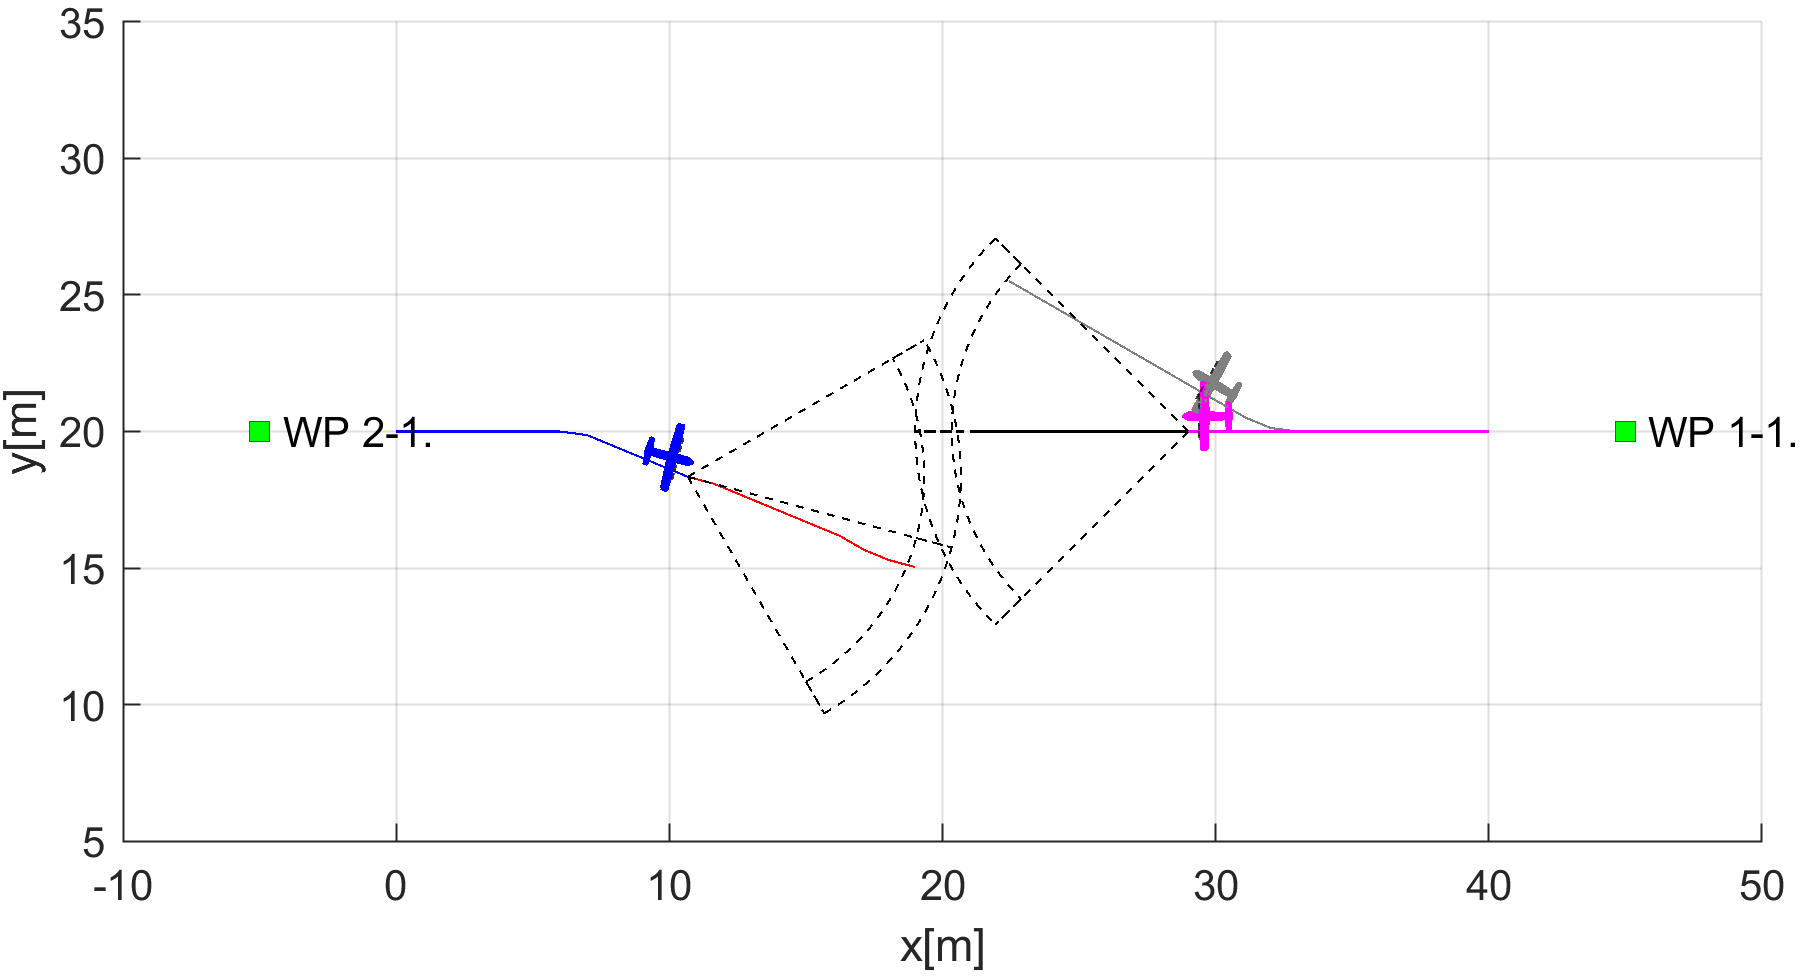
\includegraphics[width=0.9\linewidth]{\FIGDIR/NS086UTMAdversary00011}
        \caption{Deviation detection (UAS 2).}
        \label{fig:adversaryDetectedDeviation}
    \end{subfigure}
    \begin{subfigure}{0.48\textwidth}
    	\centering
        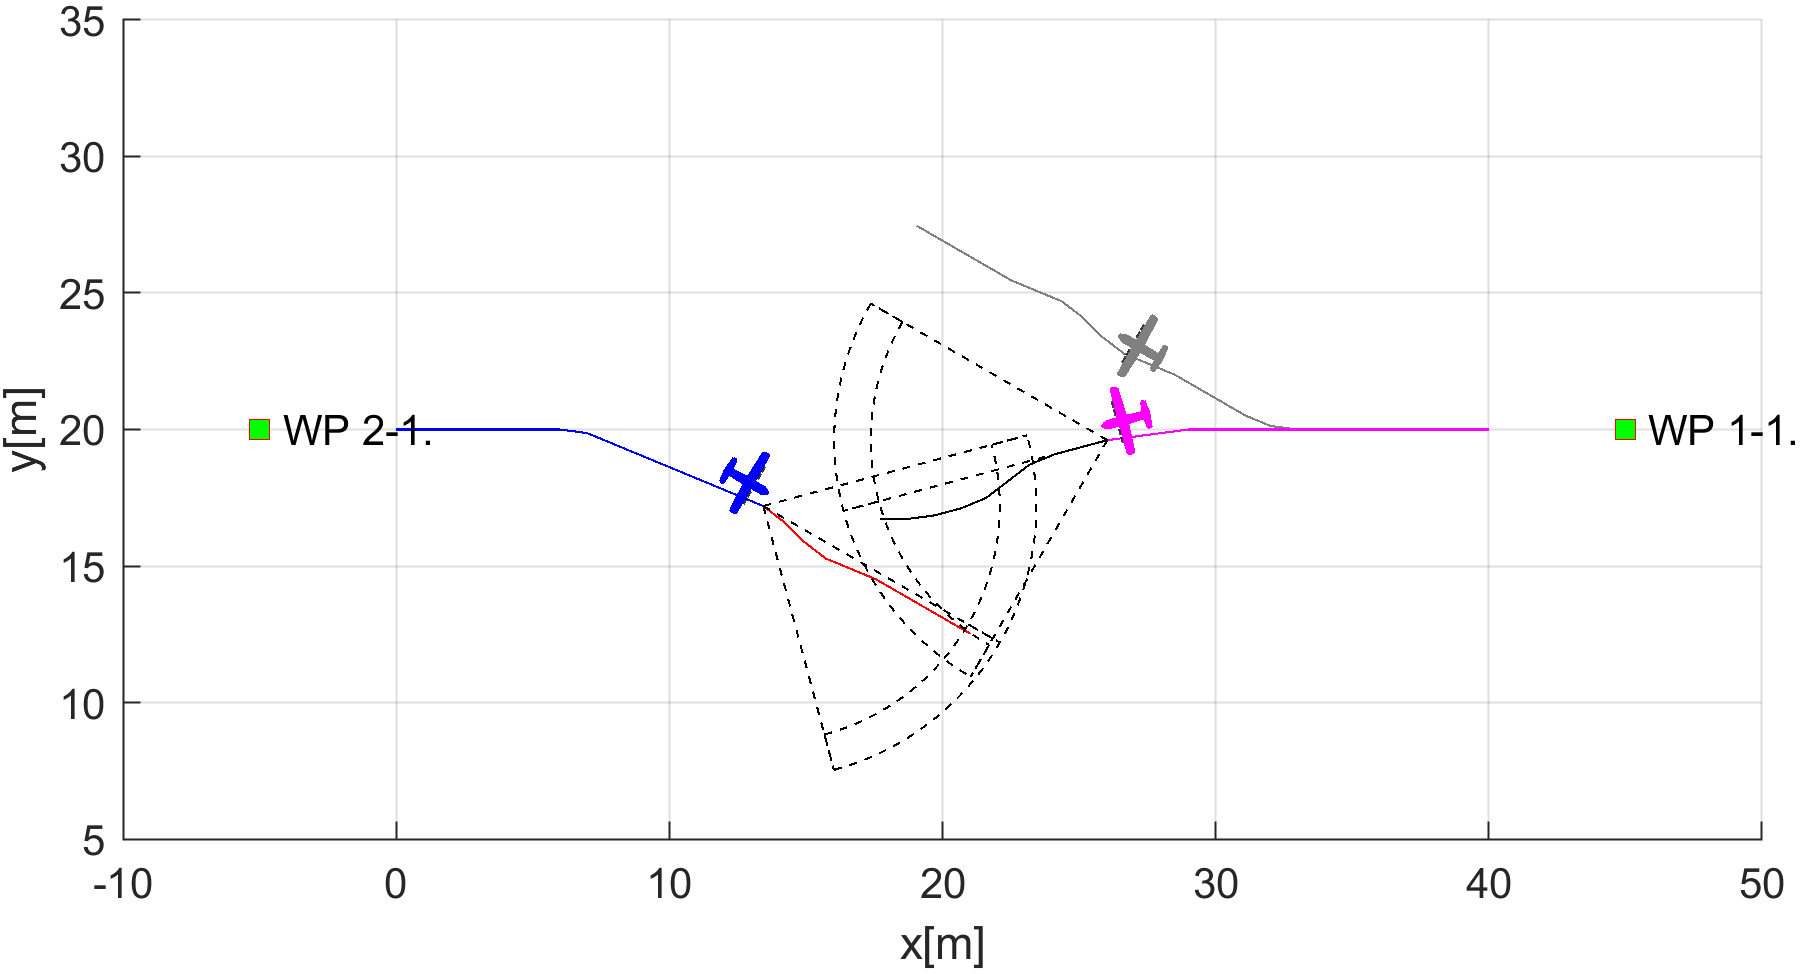
\includegraphics[width=0.9\linewidth]{\FIGDIR/NS087UTMAdversary-00014} 
        \caption{Adversary attacking (UAS 2).}
        \label{fig:adversaryAttacking}
    \end{subfigure}
    \\
    \begin{subfigure}{0.48\textwidth}
    	\centering
        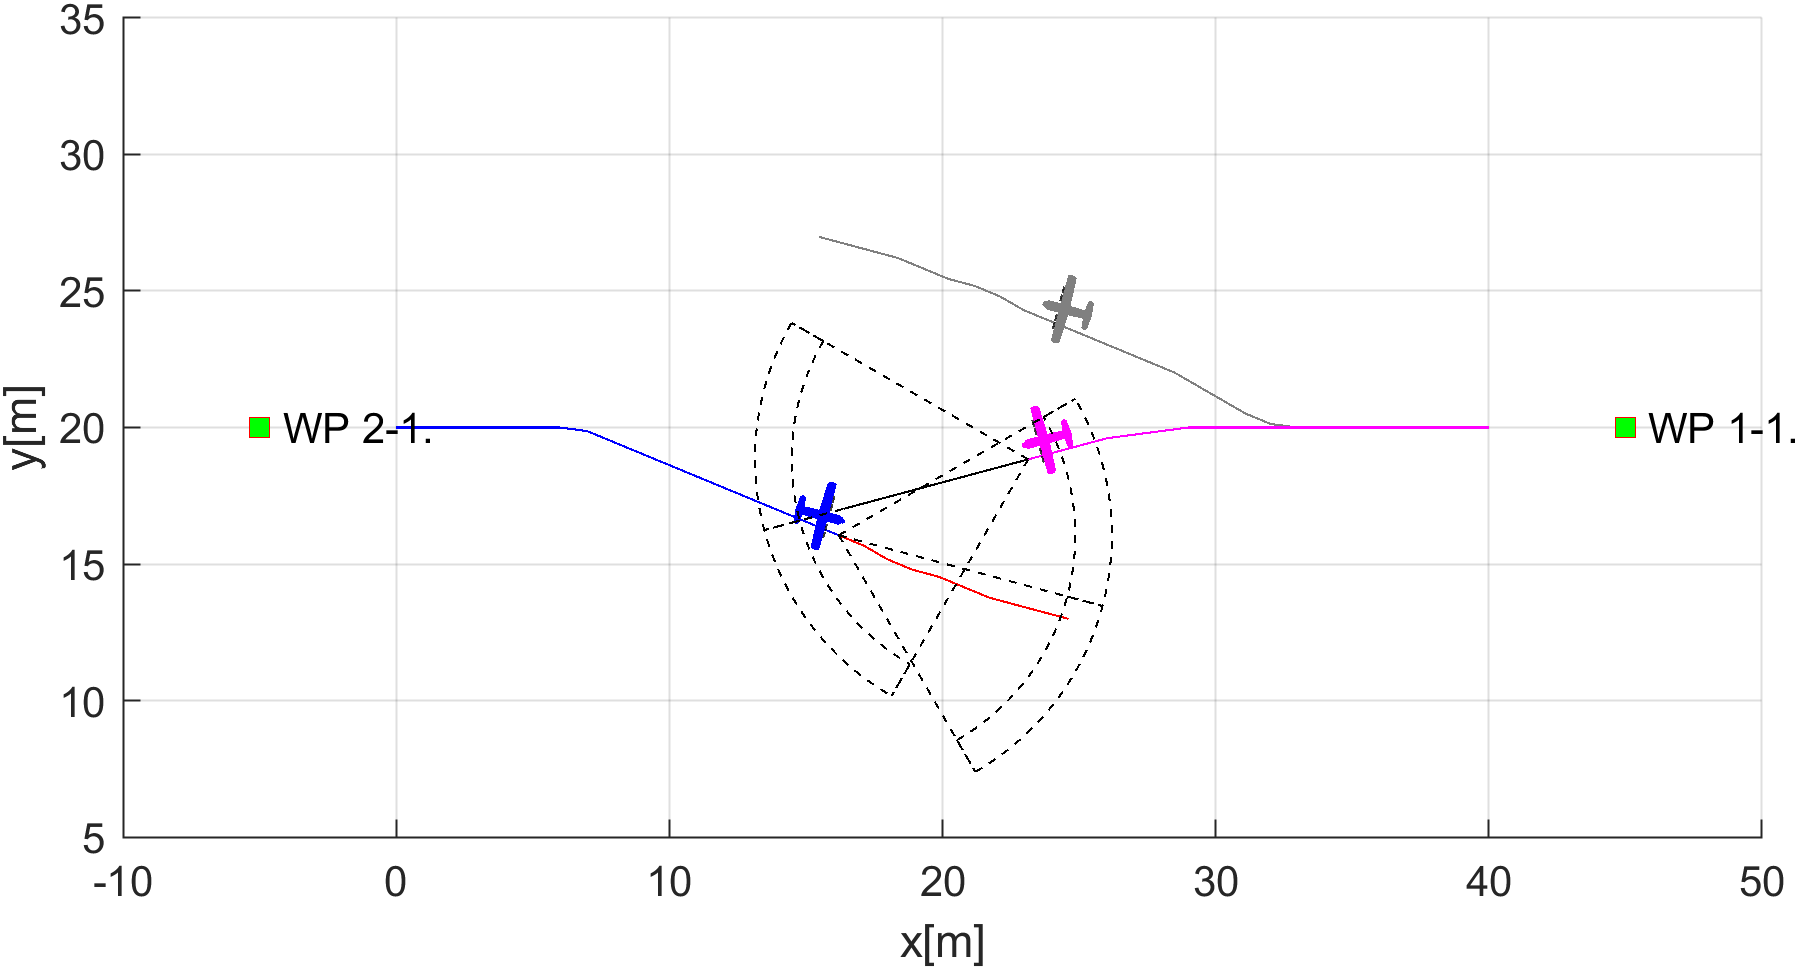
\includegraphics[width=0.9\linewidth]{\FIGDIR/NS088UTMAdversary-00017} 
        \caption{Emergency avoidance (UAS 1).}
        \label{fig:adversaryEmergencyAvoidance}
    \end{subfigure}
    \begin{subfigure}{0.48\textwidth}
    	\centering
        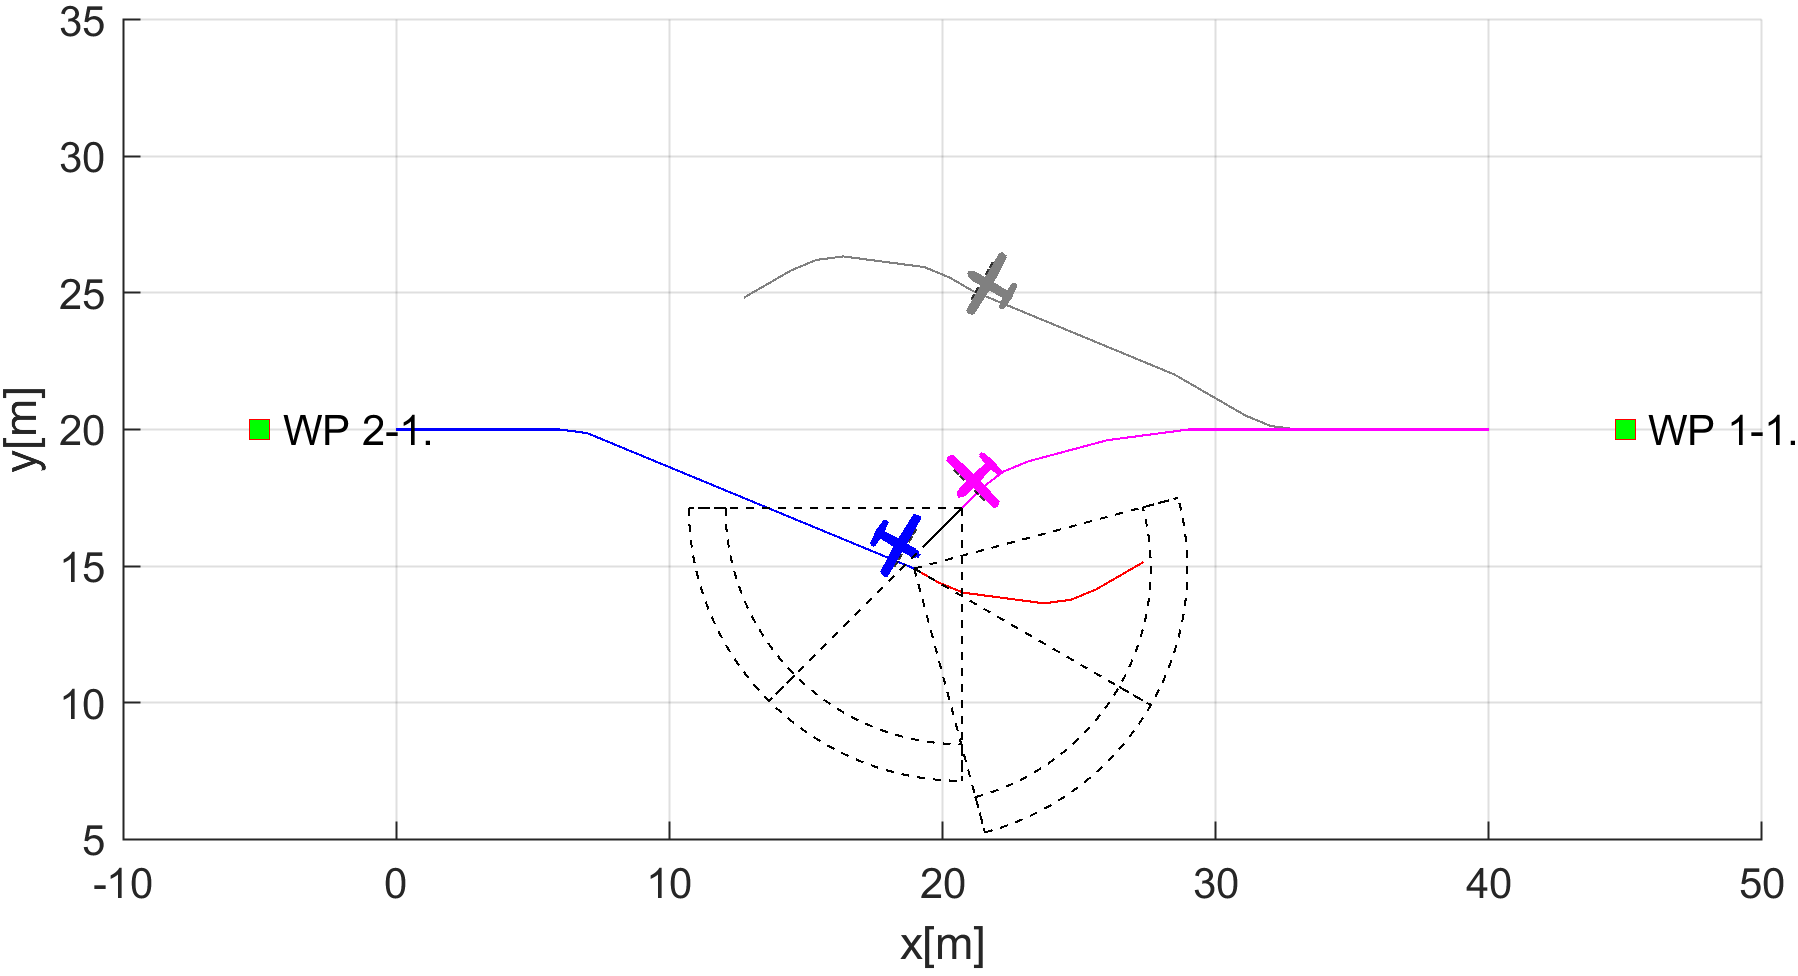
\includegraphics[width=0.9\linewidth]{\FIGDIR/NS089UTMAdversary-00020} 
        \caption{Blind spot (UAS 1).}
        \label{fig:adversaryBlindSpot}
    \end{subfigure}
    \\
    \begin{subfigure}{0.40\textwidth}
    	\centering
        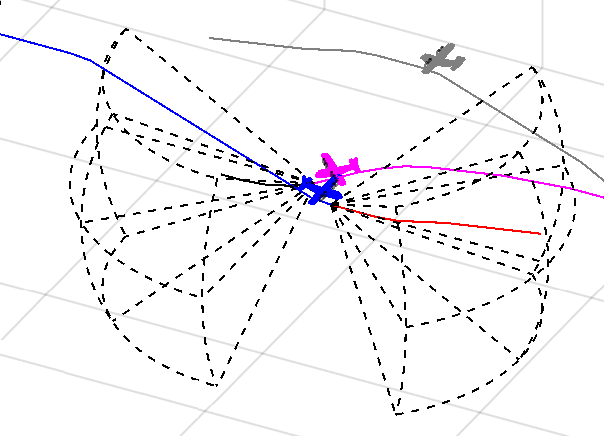
\includegraphics[width=0.9\linewidth]{\FIGDIR/NS090UTMAdversaryCrash} 
        \caption{Collision detail.}
        \label{fig:adversaryCollisionDetail}
    \end{subfigure}
    \caption{Adversarial behaviour of \emph{UAS 2} (magenta) to compliant \emph{UAS 1} (blue)}
    \label{fig:adversarialAttackNotableMoments}
\end{figure}

\paragraph{Performance Parameters Evaluation:} Performance parameters (y-axis) are tracked over \emph{UTM time} (x-axis). The evolution of \emph{performance} (fig. \ref{fig:adversaryDistanceToSafetyMargins}) is tracking following parameters:

\begin{enumerate}
    \item \emph{Expected crash distance} (gray line) - defined  as (eq . \ref{eq:crashDistance}) between UAS 1  (blue)and expected UAS 2 position (grey plane/line) over mission time $t\in[0,22]$.
    
    \item \emph{Crash distance} (blue line) - defined  as (eq . \ref{eq:crashDistance}) between UAS 1 (blue) and real UAS 2 position (magenta plane/line) over mission time $t\in[0,22]$.
    
    \item \emph{Safety margin} (yellow line) - constant value according to \emph{collision case}  (tab. \ref{tab:collisionCasesRuleBasedHeadon}) as value of \emph{10 m}. The safety margin is considered as \emph{soft constraint}.
    
    \item \emph{Body margin} (red line) - constant value according to (tab. \ref{tab:aboidanceParametersForEmergencyHeadOnScenario}) as value of  \emph{1.2 m}. The body margin is considered as \emph{hard constraint}. The breaking of \emph{body} margin means an effective \emph{collision} UAS 1 and UAS 2.
\end{enumerate}

\begin{figure}[H]
    \centering
    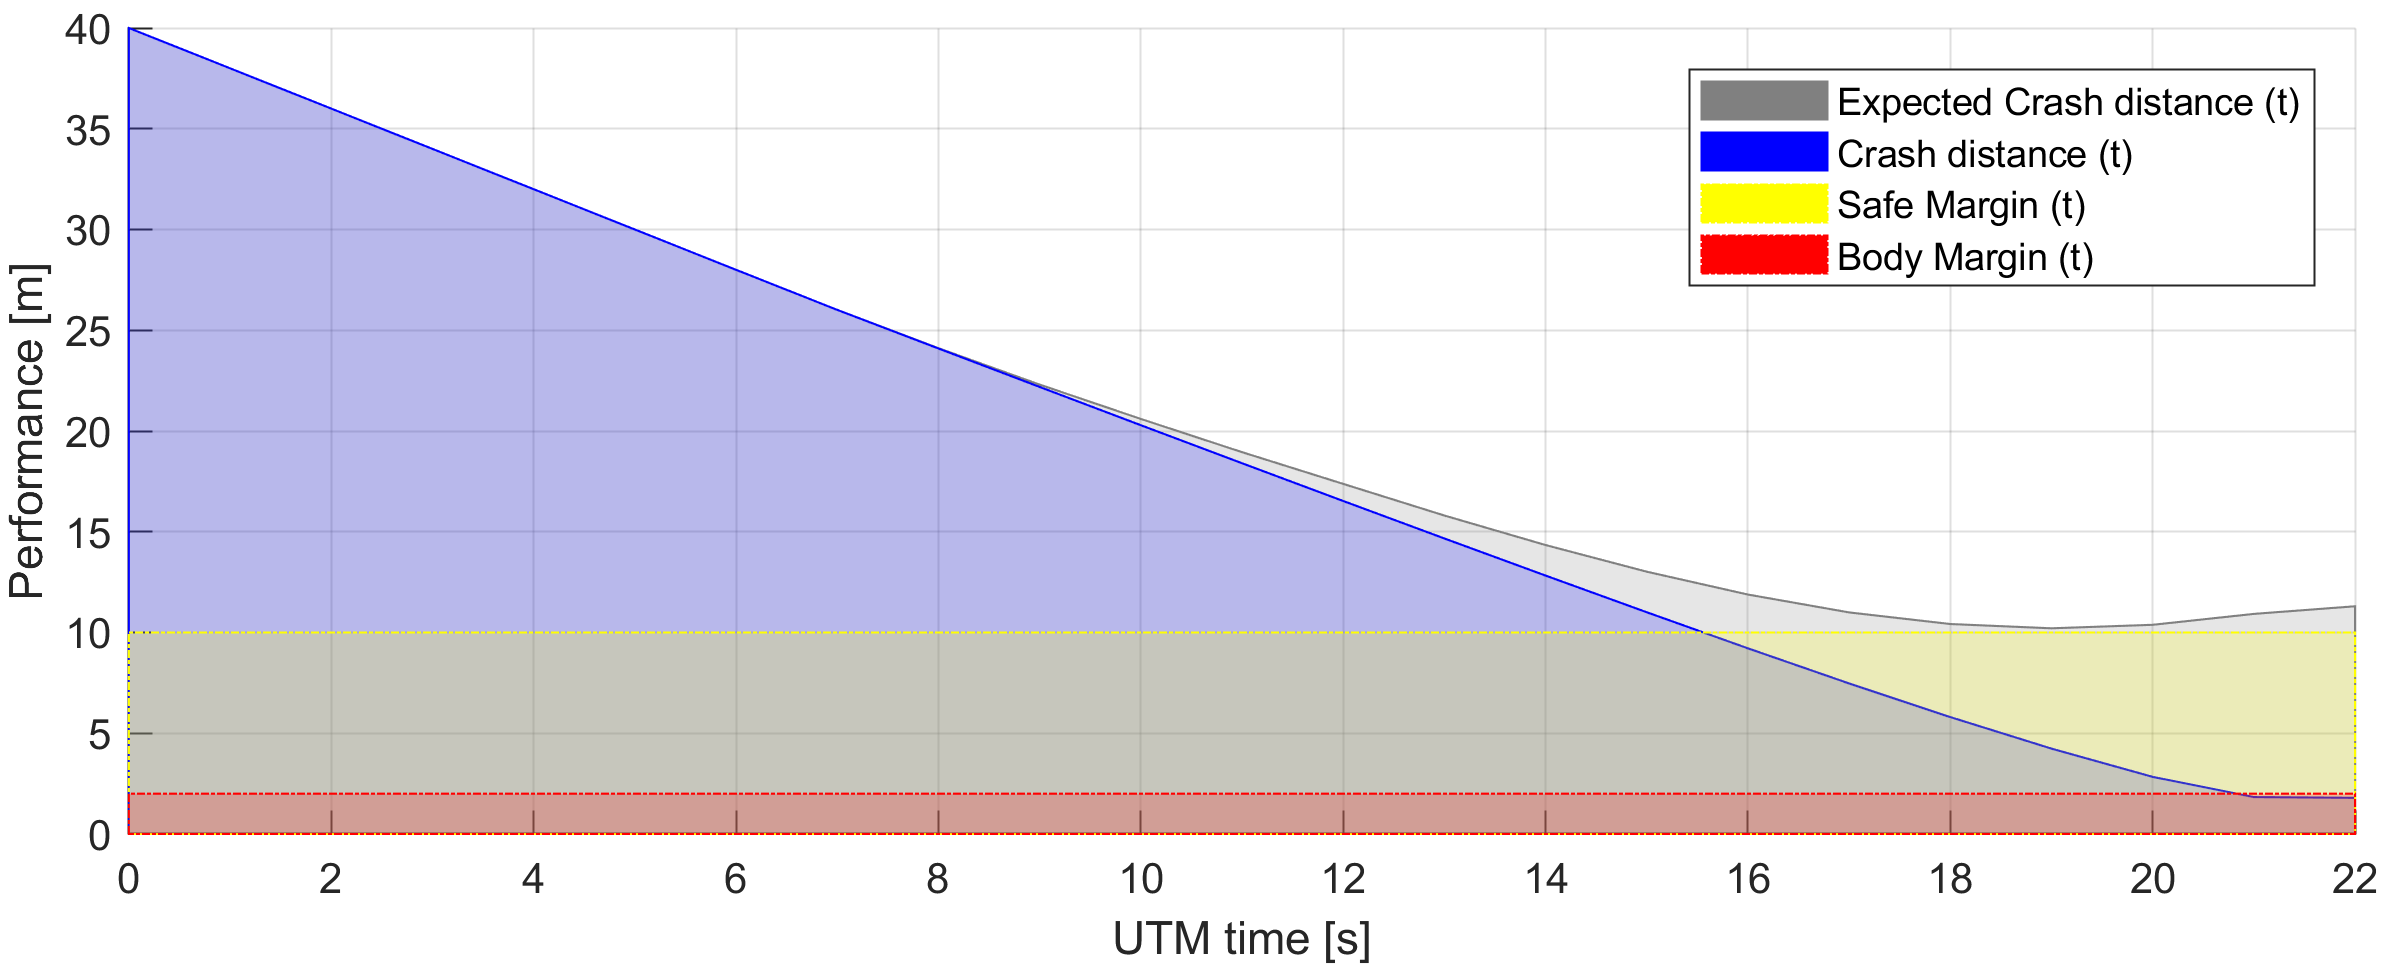
\includegraphics[width=0.95\linewidth]{\FIGDIR/NS091UTMAdversaryPerformance} 
    \caption{Expected/Real Distance to body/safety margin evolution for \emph{adversarial behaviour} of UAS 2.}
    \label{fig:adversaryDistanceToSafetyMargins}
\end{figure}

\noindent\emph{Safety criteria} for both \emph{body} and \emph{safety margins} in case of \emph{expected behaviour} are satisfied (eq. \ref{eq:expectedDistanceCondition}). This means that \emph{UAS 1} fulfilled the \emph{UTM directive} despite the fact that it entered \emph{Emergency Avoidance Mode} (fig. \ref{fig:adversaryEmergencyAvoidance}).

\begin{equation}\label{eq:expectedDistanceCondition}
    \begin{aligned}
    expectedDistanceToSafetyMargin(t) &\ge 0,\quad &\forall t \in [0,22]\\
    expectedDistanceToBodyMargin(t)  &\ge 0 \quad &\forall t \in [0,22]
    \end{aligned}
\end{equation}

\emph{Safety Margin} is broken at UTM time \emph{15 s}, \emph{body margin} is broken at UTM time \emph{21 s}, the collision happens at  UTM time \emph{22 s}. This is summarized in \emph{Distance Condition Breach} (eq. \ref{eq:distanceConditionBreach}).

\begin{equation}\label{eq:distanceConditionBreach}
    \begin{aligned}
    distanceToSafetyMargin(t) &< 0,\quad &\forall t \in [21,22]\\
    distanceToBodyMargin(t)  &< 0 \quad &\forall t \in [15,22]
    \end{aligned}
\end{equation}

\begin{note}
    An \emph{adversary behaviour} needs to be addressed on:
    \begin{enumerate}
        \item  \emph{UAS Traffic Management Level} -  our UTM implementation failed to detect \emph{deviation} (fig. \ref{fig:adversaryDetectedDeviation}) and \emph{start of attack} (fig. \ref{fig:adversaryAttacking}). UAS 2 (magenta) had clean intention from beginning and did not change pursuit even when \emph{safety margin} was breached. 
        
        \item  \emph{Emergency Avoidance Level} - our \emph{navigation loop implementation} does not consider the \emph{ill-intentions}. The UAS 1 (blue) properly switched to \emph{Emergency avoidance mode} (fig. \ref{fig:adversaryEmergencyAvoidance}) after detection of UAS2 (magenta). UAS 2 (magenta) then used the blind spot to exploit UAS 1 vulnerability.   
    \end{enumerate}
\end{note}

\newpage
\subsection{(R) Computation Footprint}\label{s:ComputaitonFootprint}

\noindent The \emph{computation footprint} is summarized in computation  load (tab. \ref{tab:computationLoadStatistics}). The \emph{computation load} (eq. \ref{eq:computationLoad}) was calculated for each \emph{time-frame} in scenarios. There is summary of \emph{minimal, maximal, average} and \emph{median} values.

The \emph{computational load} never exceed more than $55.95\%$ in case of  \emph{emergency Head On} (eq. \ref{eq:computationFeasibilityCriterion}), which means that \emph{every path} was calculated on time.

\begin{table}[H]
    \centering
    \begin{tabular}{r||r|r|r|r}
    
    \multirow{2}{*}{Scenario} & \multicolumn{4}{c}{Computation load} \\ \cline{2-5} 
    & min. & max. & avg. & med. \\ \hline\hline
    Building avoidance (fig. \ref{fig:buildingAvoidanceComputationTime})		
                            &   2.20\% &  27.40\% &  12.11\%  & 13.20\% \\\hline
    Slalom (fig. \ref{fig:slalomComputationTime})				    
                            &  12.20\% &  30.50\% &  21.42\%  & 21.50\% \\\hline
    Maze (fig. \ref{fig:mazeComputationTime})					
                            &  24.90\% &  46.10\% &  31.51\%  & 30.80\% \\\hline
    Storm (fig. \ref{fig:stormComputationTime})					
                            &   2.60\% &  26.90\% &  11.57\%  & 13.90\% \\\hline\hline
    
    Emergency Converging (fig. \ref{fig:emergencyConvergingComputationTime})    
                            &   2.75\% &  16.50\% &   5.84\%  &  4.95\% \\\hline
    Emergency Head On (fig. \ref{fig:emergencyHeadOnComputationTime})	 	
                            &	3.90\% &  55.95\% &  13.19\%  &  6.90\% \\\hline
    Emergency Multiple (fig. \ref{fig:emergencyHeadOnMultipleComputationTime})	 	
                            &	5.90\% &  52.35\% &  12.77\%  &  8.56\% \\\hline\hline
    
    Rule-based Converging (fig. \ref{fig:ruleBasedCConvergingComputationTime})	
                            &   3.60\% &  13.50\% &   7.32\%  &  5.97\% \\\hline
    Rule-based Head on (fig. \ref{fig:ruleBasedHeadOnComputationTime})		
                            &   4.65\% &  41.60\% &  13.64\%  &  9.30\% \\\hline
    Rule-based Multiple	(fig. \ref{fig:ruleBasedMultipleComputationTime})	
                            &   4.37\% &  23.30\% &  11.96\%  & 10.93\% \\\hline
    Rule-based Overtake	(fig. \ref{fig:ruleBasedOvertakeComputationTime})	
                            &   3.85\% &  13.40\% &   7.62\%  &  6.70\% 
    
    \end{tabular}
    \caption{\emph{Computation load statistics} for all test cases.}
    \label{tab:computationLoadStatistics}
\end{table}

\noindent \emph{Following observations can be made:}

\begin{enumerate}
    \item \emph{Building avoidance}, \emph{Slalom}, and \emph{Maze} scenarios - the computation load is increasing with the \emph{amount of static obstacles}. The \emph{average load} for \emph{Emergency avoidance mode} in \emph{clustered environment} is $31.51\%$ (Maze).
    
    \item \emph{Storm scenario} - the overall \emph{computation load} is very low due the \emph{moving constraint implementation} (sec. \ref{s:MovingVirtualConstraints}).
    
    \item\emph{Emergency Converging/Head On/Multiple} scenarios - the \emph{overall computation load} is quite high due the ineffective \emph{body volume intersection} (sec. \ref{s:bodyvolumeIntersection}) implementation.
    
    \item \emph{Rule-based Converging/Head On/Multiple} scenarios - the \emph{median computational} load is low, because of the linear \emph{rule implementation} (sec. \ref{sec:ruleImplementation})
    
    \item \emph{Rule-based Overtake} - the \emph{average computation load} is very low, because only \emph{divergence/convergence} (rule. \ref{tab:ruleOvertakeDefinition}) waypoints are calculated and UAS stays in \emph{navigation mode}.
\end{enumerate}
   

%% This adds a line for the Bibliography in the Table of Contents.
\addcontentsline{toc}{chapter}{Bibliography}
%% *** Set the bibliography style. ***
%% (change according to your preference/requirements)
%\bibliographystyle{plain}
%% *** Set the bibliography file. ***
%% ("thesis.bib" by default; change as needed)
\bibliography{thesis}

%% *** NOTE ***
%% If you don't use bibliography files, comment out the previous line
%% and use \begin{thebibliography}...\end{thebibliography}.  (In that
%% case, you should probably put the bibliography in a separate file and
%% `\include' or `\input' it here).

\end{document}
